\section{Methods and Materials}

\subsection{ANTs volumetric-based cortical thickness estimation pipeline}

The ANTs-based cortical thickness estimation workflow is illustrated 
in Figure \ref{fig:pipeline}.  The steps are as follows:
\begin{enumerate}
  \item initial N4 bias correction on input anatomical MRI,
    \textcolor{blue}{do you usually bias correct the raw image?  phil
      had some problems with the automated (otsu) masking employed
      therein .... esp with elderly brain}
  \item brain extraction using a hybrid segmentation/template-based strategy,
  \item alternating between prior-based segmentation and white matter posterior
        probability weighted bias correction,
  \item DiReCT-based cortical thickness estimation, and
  \item optional normalization to specified template.
\end{enumerate}
Each component, including both software and data, is briefly detailed 
below with the relevant references for additional information. 


%We also note that each component is publicly available with all ANTs 
%algorithms available as open source.%
%\footnote{
%http://www.picsl.upenn.edu/ANTS
%}
Additionally, the coordination of all the algorithmic components is
encapsulated in the shell script \verb#antsCorticalThickness.sh#.  This includes
optimal parameters for each of the algorithmic components which has worked
well for our processing and which are used to acquire the results 
described in this work.

%\lstset{frame = tb,
%        framerule = 0.25pt,
%        float,
%        fontadjust,
%        backgroundcolor={\color{listlightgray}},
%        basicstyle = {\ttfamily\scriptsize},
%        keywordstyle = {\ttfamily\color{listkeyword}\textbf},
%        identifierstyle = {\ttfamily},
%        commentstyle = {\ttfamily\color{listcomment}\textit},
%        stringstyle = {\ttfamily},
%        showstringspaces = false,
%        showtabs = false,
%        numbers = none,
%        numbersep = 6pt,
%        numberstyle={\ttfamily\color{listnumbers}},
%        tabsize = 2,
%        language=,
%        floatplacement=!h,
%        caption={\small \baselineskip 12pt DiReCT long command line menu which is invoked using the `{\ttfamily {-}{-}help}' option.  The short command line menu is obtained by typing `{\ttfamily {-}h}'}.,
%        captionpos=b,
%        label=listing:long
%        }
%\lstsetcpplong
%\begin{lstlisting}
%This script, apb.sh, performs T1 anatomical brain 
%processing where the following steps are currently 
%applied:
%
%  1. Brain extraction
%  2. Brain 3-tissue segmentation
%  3. Cortical thickness
%  4. (Optional) registration to a template
%
%Usage:
%
%abp.sh -d ImageDimension
%       -i T1Image.nii.gz
%       -e BrainExtractionTemplate
%       -m BrainExtractionProbabilityMask
%       -l BrainParcellationTemplate
%       -p BrainParcellationProbabilityMask
%       <OPTARGS>
%       -o OutputPrefix
%
%Example:
%
%abp.sh -d 3 
%       -i t1.nii.gz 
%       -e brainWithSkullTemplate.nii.gz 
%       -m brainPrior.nii.gz 
%       -l corticalLabels.nii.gz 
%       -p corticalLabelPriors.nii.gz 
%       -o output
%
%Compulsory arguments:
%
%     -d:  ImageDimension                        2 or 3 (for 2 or 3 dimensional single image)
%     -a:  Anatomical T1 image                   typically T1.
%     -e:  Brain extraction template             Anatomical template created using e.g. LPBA40 data set with
%                                                buildtemplateparallel.sh in ANTs.
%     -m:  Brain extraction probability mask     Brain probability mask created using e.g. LPBA40 data set which
%                                                have brain masks defined, and warped to anatomical template and
%                                                averaged resulting in a probability image.
%     -l   Brain segmentation template           Anatomical template for brain segmentation.  E.g. NIREP template
%                                                with labels.
%     -p   Brain segmentationpriors              Label probability priors corresponding to the image specified
%                                                with the -l option.  Specified using c-style formatting, e.g.
%                                                -p labelsPriors\%02d.nii.gz.
%     -o:  OutputPrefix                          The following images are created using the specified prefix:
%                                                  * /Users/ntustison/Data//tmp13243//tmpN4Corrected.nii.gz
%                                                  * /Users/ntustison/Data//tmp13243//tmpExtractedBrain.nii.gz
%                                                  * /Users/ntustison/Data//tmp13243//tmp3TissueBrainSegmentation.nii.gz
%                                                  * /Users/ntustison/Data//tmp13243//tmpCorticalThickness.nii.gz
%                                                  * /Users/ntustison/Data//tmp13243//tmpSurfaceCurvature.nii.gz
%
%Optional arguments:
%
%     -s:  image file suffix                     Any of the standard ITK IO formats e.g. nrrd, nii.gz (default), mhd
%     -t:  template for t1 registration
%     -k:  keep temporary files                  Keep brain extraction/segmentation warps, etc (default = false).
%     -w:  white matter label                    white matter label for segmentation (default = 3).
%     -g:  gray matter label                     cortical gray matter label for segmentation (default = 2)
%     -i:  max iterations for registration       ANTS registration max iterations (default = 50x100x20)
%\end{lstlisting}



\begin{figure*}
  \centering
  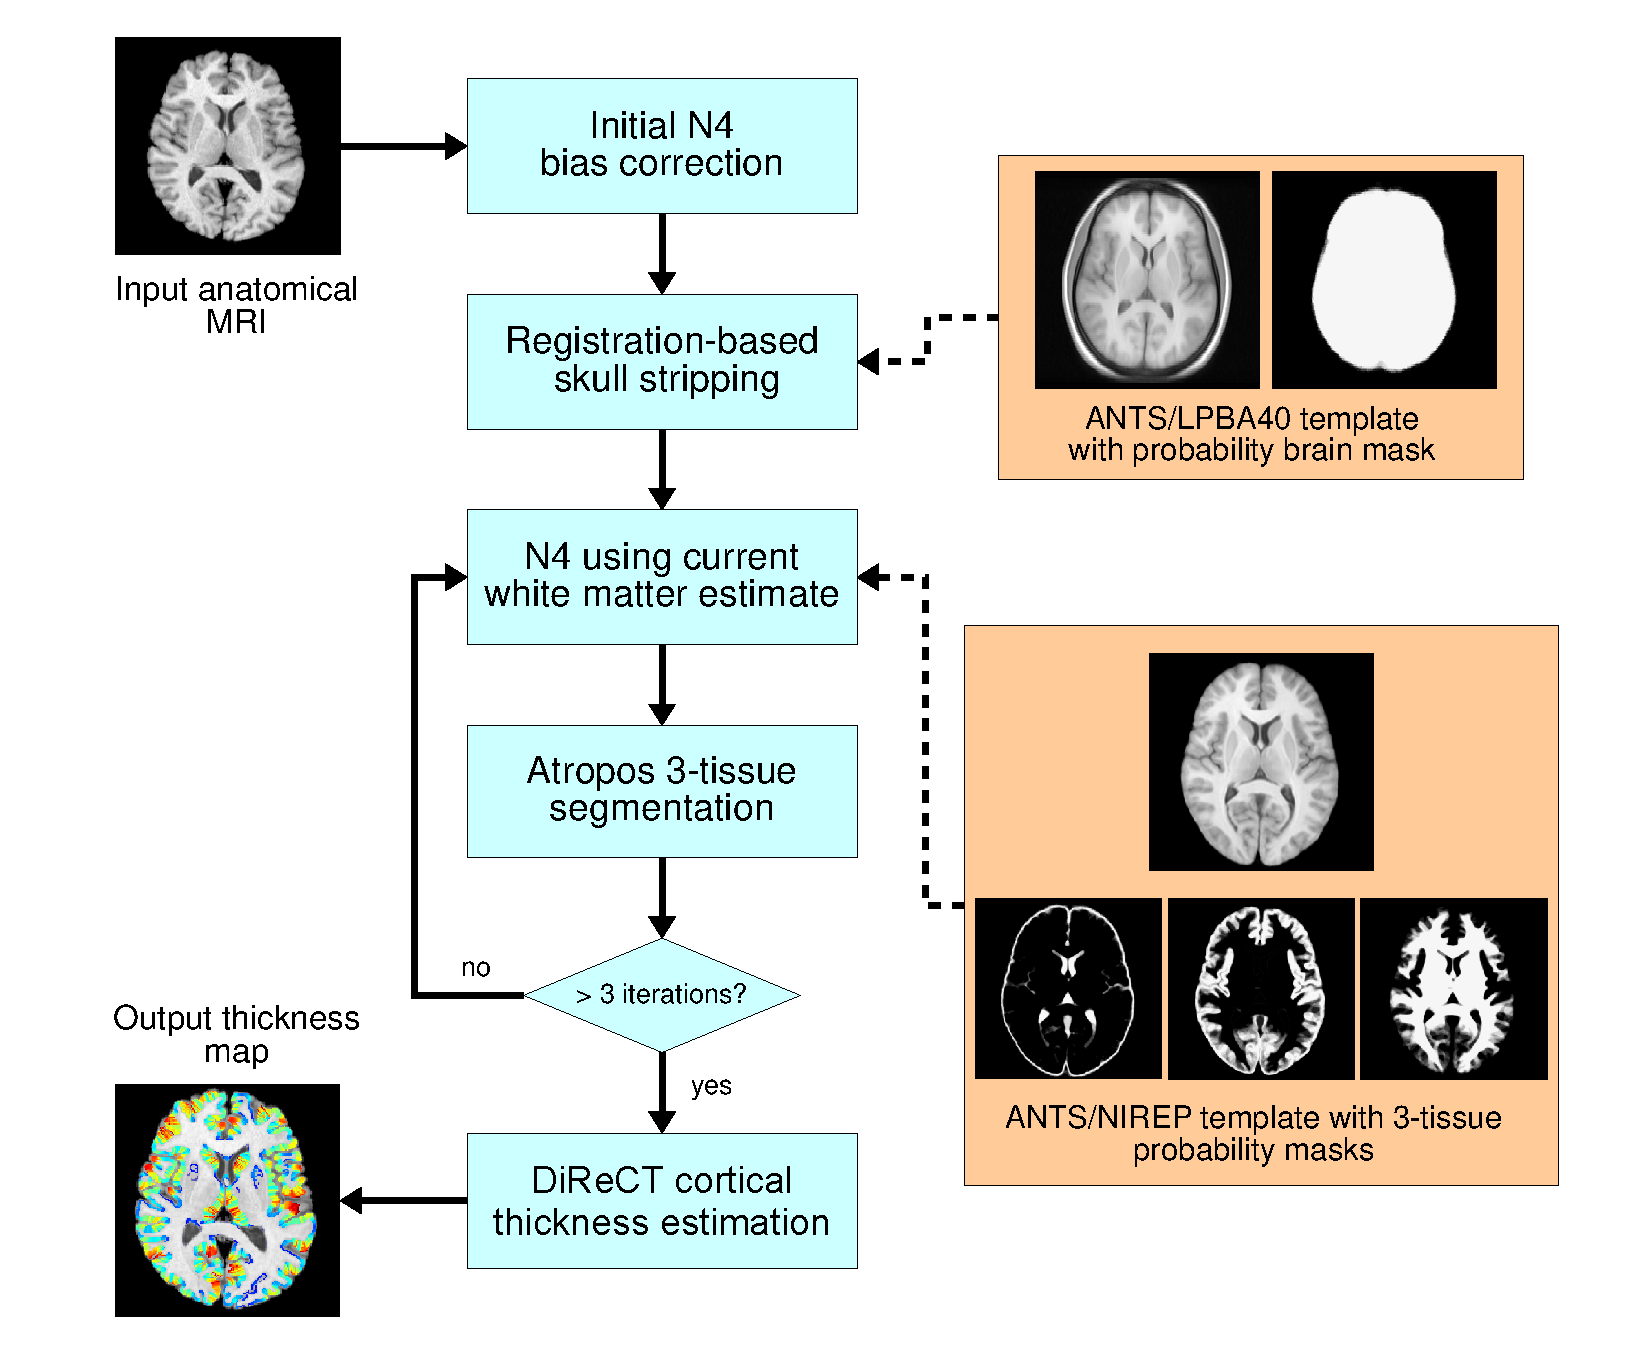
\includegraphics[width=130mm]{Figures/Kapowski_pipeline.pdf}
  \caption{The ANTs T1 processing workflow containing all elements for 
  determining cortical thickness. Not shown is the optional single subject
  to template registration.}
  \label{fig:pipeline}
\end{figure*}

\subsubsection{Anatomical template construction}

Normalizing images to a standard coordinate system
reduces intersubject variability in population studies.  Various
approaches exist for determining the normalized space such as the selection
of a pre-existing template based on a single subject, e.g. the Talairach
atlas \citep{Talairach1988}, or a publicly available averaged group of
subjects, e.g. the MNI \citep{Collins1994} or ICBM \citep{Mazziotta1995}
templates.  Additionally, mean templates constructed from labeled
data can be used to construct spatial priors for improving segmentation
algorithms.
The work of \cite{avants2010} explicitly models the geometric component of the 
normalized space during optimization to produce such mean templates.  Coupling the intrinsic symmetry of 
SyN pairwise registration \citep{avants2011} and an
optimized shape-based sharpening/averaging of the template appearance, Symmetric Group
Normalization (SyGN) is a powerful framework for producing optimal population-specific
templates \citep{avants2010} with arbitrary similarity metric choice.  

%One challenge with standard templates is that they may inadvertently bias one's results by enabling better normalization of subjects to which the template is more similar.  This issue is exacerbated when dealing with populations that have high variance (e.g. due to disease) and/or when one's normalization method is low-dimensional (not flexible enough to capture large shape differences). 

%Population-specific templates alleviate some of
%the issues with other template approaches by deriving a most representative image from the population
%\citep{Good2001}.  Large deformation registration algorithms also reduce
%this confound by being less sensitive to the deformation distance
%between subject and target.  Some approaches combine both advantages,
%for instance, the diffeomorphic approach of Joshi et al. employs the
%SSD metric and a shape distance to bring the subject group of images
%into alignment \citep{Joshi2004}.  Variants
%include extension to multiple modalities \citep{Lorenzen2006} and small deformations
%\citep{Geng2009}.  These approaches iteratively minimize group difference in ``congealing''
%towards a representative image template \citep{Learned-Miller2006}.


The ANTs implementation of this technique is currently available as a shell script, 
\verb#buildtemplateparallel.sh#, and a multivariate version,
\verb#antsMultivariateTemplateConstruction.sh#, both of which are distributed as part of
 the ANTs repository.
The latter script permits the construction of multimodal templates (e.g. 
T1-weighted, T2-weighted, and proton density MRI as described in the 
Evaluation section).  Both scripts accommodate a variety of computational resources
for facilitating template construction.  These computational resource possibilities include:
\begin{itemize}
  \item serial processing on a single workstation, 
  \item parallelized processing on a single workstation with multiple cores using \verb#pexec#%
  \footnote{http://www.gnu.org/software/pexec/pexec.1.html},
  \item parallelized processing using Apple's XGrid technology%
  \footnote{https://developer.apple.com/hardwaredrivers/hpc/xgrid\_intro.html}, 
  \item parallelized processing using Sun Grid Engine for cluster-based systems%
  \footnote{http://www.oracle.com/technetwork/oem/grid-engine-166852.html}, and 
  \item parallelized processing using the Portable Batch System for cluster-based systems%
  \footnote{http://www.pbsworks.com/}.
\end{itemize}
Within this work multiple templates were created for all stages of 
image processing and analysis.  The creation of these templates are described
in the corresponding data section.

\textcolor{blue}{what is the motivation of the multivar template here?
  it would seem useful to add an FA component to the segmentation step
  to aid in cortical / wm delineation which would motivate the
  multivar template approach but might be difficult to establish that
  this actually helps .... though we could compare both ways : univar
  and multivar }

%Given a set of representative images, 
%$\{I_1, I_2, \ldots, I_M\}$, optimization involves finding the set of paired
%diffeomorphic transformations, $\left\{\left(\phi^1_1, \phi^1_2\right), 
%\left(\phi^2_1, \phi^2_2\right), \ldots, \left(\phi^M_1, \phi^M_2\right) \right\}$,
%the optimal template appearance, $J^*$, and corresponding coordinate system, $\psi(\mathbf{x})$,
%which minimize the following cost function:
%\begin{align}
%  \sum_{m=1}^M \left[
%    D\left( \psi(\mathbf{x}), \phi^m_1(\mathbf{x}, 1) \right) + 
%    \Pi \left( I_m\left(\phi^m_2(\mathbf{x}, 0.5) \right), J^*\left(\phi^m_1(\mathbf{x}, 0.5) \right) \right)
%    \right]
%\end{align}
%where $D$ is the diffeomorphic shape distance, 
%\begin{align}
%  D\left(\phi(\mathbf{x}, 0), \phi(\mathbf{x}, 1)\right) = \int_{0}^1 \| v(\mathbf{x}, t) \|_L dt, 
%\end{align}
%dependent upon the choice of the linear operator, $L$, and
%$v$ is the diffeomorphism-generating velocity field, 
%\begin{align}
%  v\left(\phi(\mathbf{x}, t), t \right) = \frac{d\phi(\mathbf{x}, t)}{dt},\,\,\, \phi(\mathbf{x}, 0) = \mathbf{x}.
%\end{align}
%$\Pi$ is th
%e choice of similarity metric, often cross-correlation \citep{Avants2008a}, calculated in the 
%virtual domain midway between each individual image and the current estimate of the template. 
%
%With initial assignment of $\left\{\left(\phi^m_1, \phi^m_2\right)\right\}$ and $\psi(\mathbf{x})$ 
%to identity, iterative optimization
%involves estimating the pairwise transformations, estimation of the optimal template appearance, and 
%updating $\psi(\mathbf{x})$ by averaging the current estimate of $\left\{\phi_1^m\right\}$.  


\subsubsection{N4 Bias field correction}

Critical to quantitative processing of MRI is the minimization of
field inhomogeneity effects which causes artificial low frequency 
intensity variation across the image.  Large-scale studies, such
as the Alzheimer's Disease Neuroimaging Initiative (ADNI), employ
perhaps the most widely used bias correction algorithm, N3 \cite{sled1998}, 
as part of their standard protocol \citep{boyes2008}.

In \cite{tustison2010}, we introduced an extension of N3, denoted as
N4, which demonstrates improved performance and convergence behavior
on a variety of data.  This improvement is a result of an enhanced 
fitting routine (which includes multi-resolution capabilities) and a modified optimization 
formulation.  For our workflow, the additional possibility of specifying
a weighted mask in N4 permits the use of the current white matter probability map 
calculated during the segmentation pipeline for further improvement of 
bias field estimation.  In addition to its public availability 
through ANTs and the Insight Toolkit, it has also been included in
the popular open source Slicer software package for visualization and medical
image computing \cite{fedorov2011}.

N4 is used in two places during the individual subject processing (cf. Figure
\ref{fig:pipeline}).  Following conversion of the raw dicom T1-weighted image
to Nifti format using our related \verb#Neuropipedream# set of raw image conversion
and organization tools%
\footnote{
http://sourceforge.net/projects/neuropipedream/
}, N4 is used to generate an initial bias corrected image for use in
brain extraction.  The input mask is created by adaptively thresholding 
the background from the foreground using Otsu's algorithm \cite{otsu1979}.
Following brain extraction, the three-tissue segmentation involves iterating
between bias field correction using the current white matter posterior 
probability as a weight mask and then using that bias corrected image
as input to the Atropos segmentation step (described in subsequent sections). 

\subsubsection{Atropos 3-tissue segmentation}

In \cite{avants2011a} we presented an open source $n$-tissue segmentation software tool
(which we denote as ``Atropos'') attempting to distill 20+ years of active research in this area
particularly some of its most seminal work (e.g. \cite{zhang2001,ashburner2005}). 
Specification of prior probabilities includes spatially varying Markov Random Field modeling, 
prior label maps, and prior probability maps typically derived from our template building 
process.  Additional
capabilities include handling of multivariate data, 
partial volume modeling \cite{shattuck2001}, a memory-minimization mode,
label propagation, a plug-n-play architecture for incorporation of novel likelihood models
which includes both parametric and non-parametric models for both scalar and tensorial
images, and alternative posterior formulations for different segmentation tasks.

\subsubsection{Brain extraction}

Brain extraction using ANTs combines template building, high-performance
brain image registration \citep{avants2011}, and Atropos with topological refinements.  
An optimal template for brain extraction is 
generated offline using labeled brain data.  For example, in this work we use the LPBA40 data 
for generating a brain extraction template and a corresponding brain probability mask which is
available on the website associated with this submission. 

  The warped template probability map is thresholded at 0.5 and the resulting mask is dilated
with a radius of 2.  Atropos is used to generate an initial 3-tissue segmentation estimate within the mask
region.  Each of the three tissue masks undergo specific morphological operations which are then
combined to create a brain extraction mask for use in the rest of the
cortical thickness workflow.  \textcolor{blue}{does there need to be a
  bit more technical detail here?  while you can refer to the script,
  why perform these operations?  there are numerous references, most
  germane probably some recent stuff from J Prince ( i think ) and the
  freesurfer watershed approach which came from ... i forget ... maybe
  one of the french groups.}

A comparison using open access brain data with publicly available
brain extraction algorithms including AFNI's \verb#3dIntracranial#
\citep{ward1999}, FSL's \verb#BET2# \citep{smith2002}, Freesurfer's
\verb#mri_watershed# \citep{segonne2004}, and BrainSuite
\citep{dogdas2005} demonstrated that our combined
registration/segmentation approach \citep{avants2010a} performs at the
top level alongside BrainSuite (tuned) and FreeSurfer.
\textcolor{blue}{ok you have the segonne ref here ... }


\subsubsection{DiReCT Cortical Thickness Estimation}

Although the basic formulation of DiReCT as reported in this work is as it 
was introduced in \cite{das2009}, we have made several 
improvements.  Perhaps the most significant advance is that this particular 
ITK-compatible implementation has been significantly multi-threaded,
is written in ITK coding style, and has been made publicly available through 
ANTs complete with a unique user interface design developed specifically for 
ANTs tools.  

\subsection{Public Data Resources}

\subsubsection{LPBA40 Data for Skull Stripping}

For the brain extraction step
we used the data from the LPBA40 repository \citep{shattuck2008}.
These data consist of 40 high-resolution 3D Spoiled Gradient Echo
(SPGR) MRI acquisitions which were manually labeled delineating
56 brain structures.  Additional post processing 
included automated brain extraction using FSL's brain extraction tool 
\citep{smith2002} which was followed by manual corrections.  These
40 brain masks are also included with the database.  

All 40 subjects were used to create a population-specific
unbiased average template \cite{avants2010}.  The brain masks corresponding 
to the 20 subjects were warped to the template space using the 
transforms derived during the template building process.  A template 
probability mask was created by averaging the warped brain masks.
For brain extraction of any single individual this ANTS-based LPBA40 template 
is coarsely registered to the single subject brain.  The template
probability brain mask is warped to the individual subject and 
is used as the initial brain mask estimate.  As mentioned previously,
Atropos and binary morphological operations are used to refine the
brain mask estimate.

\subsubsection{NIREP Data for 3-Tissue Segmentation}

The nonrigid image registration evaluation project is an ongoing 
framework for evaluating image registration algorithms \citep{christensen2006}.
The initial data set introduced into the project consists of 
16 (8 male and 8 female) high resolution skull-stripped brain 
data with 32 cortical labels manually drawn using published protocol.
Given the gray matter labels, the white matter and CSF were identified 
for each of the 16 subjects using Atropos.  Similar to the LPBA40
data set, a NIREP template was created from all 16 subjects and each the
warped labels were used to create probabilistic estimates of the 
labeled region boundaries. These probability maps were used as 
spatial prior probabilities during the 3-tissue segmentation component
of the pipeline.  Using SyN, the NIREP template is registered to the
extracted individual subject brain which is followed by a warping of the 
NIREP priors to the space of the individual subject.  The initial warped 
white matter probability map is used as the weighted confidence mask 
in the follow-up bias correction step.

\subsection{IXI Data for Pipeline Evaluation}

The IXI data%
\footnote{
http://biomedic.doc.ic.ac.uk/brain-development/
}
consists of approximately 600 healthy subjects imaged at three sites 
using several modalities (T1-weighted, T2-weighted, proton density, magnetic 
resonance angiography, and diffusion tensor imaging).  The 
database also consists of  demographic information such as age, weight,
height, ethnicity, occupation category, educational level, and marital status.
The number of subjects spanning a range of demographic characteristics makes
this a rich data set for validating and exploring correlations with cortical 
thickness measured using the ANTs pipeline.

\begin{figure}
  \centering
  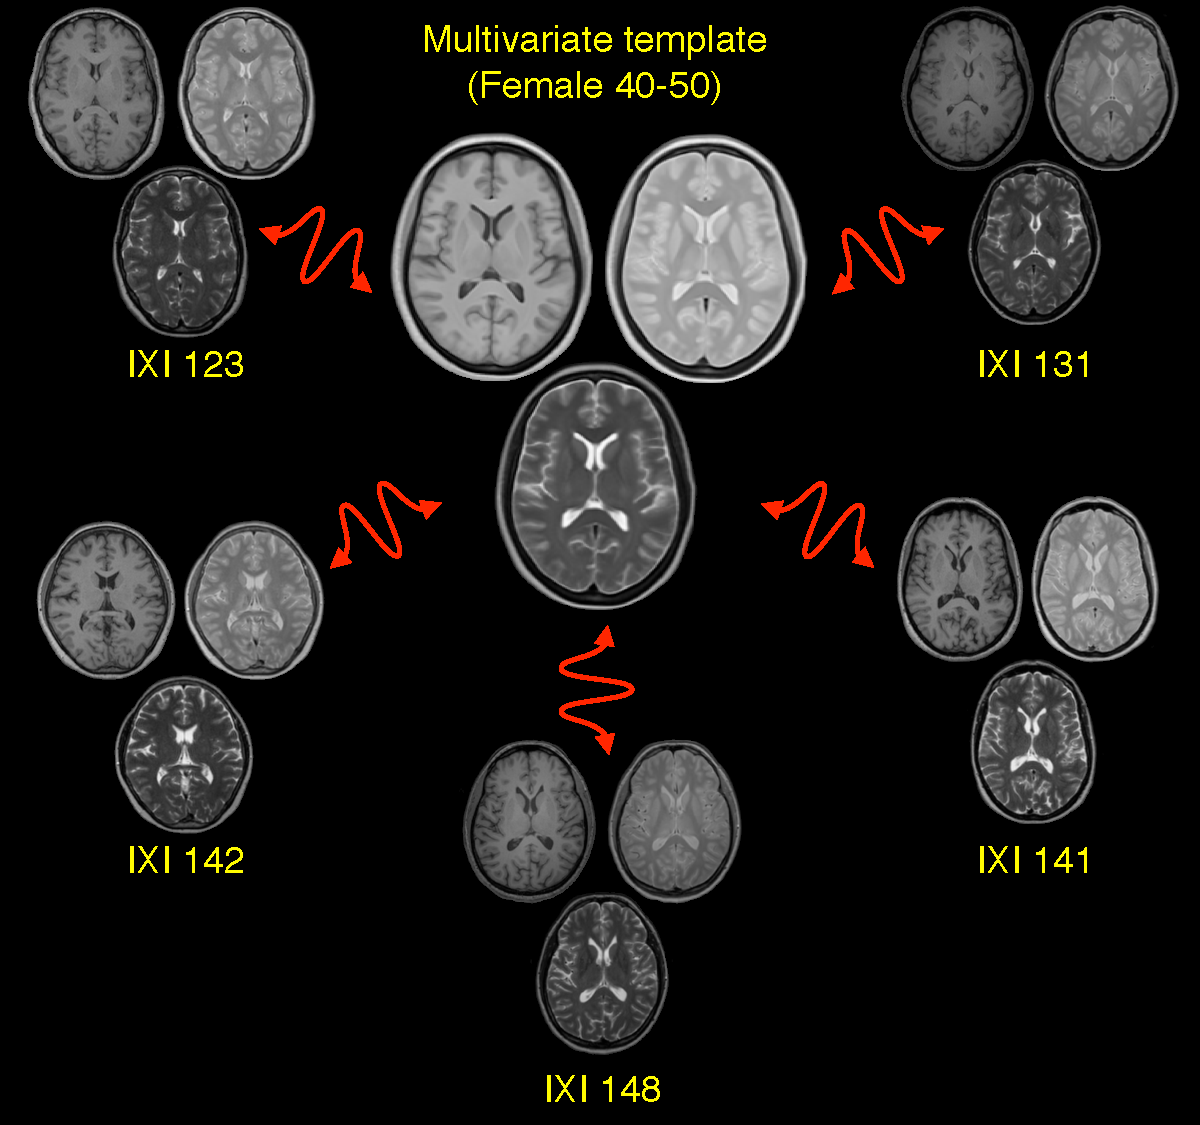
\includegraphics[width=90mm]{Figures/template.pdf}
  \caption{Sample multivariate template constructed from a subset of the IXI data (female, age 40--50).  Axial slices of five of the 37 total subjects from this cohort are shown. }
  \label{fig:template}
\end{figure}

